% Template for Cogsci submission with R Markdown

% Stuff changed from original Markdown PLOS Template
\documentclass[10pt, letterpaper]{article}

\usepackage{cogsci}
\usepackage{pslatex}
\usepackage{float}
\usepackage{caption}

% amsmath package, useful for mathematical formulas
\usepackage{amsmath}

% amssymb package, useful for mathematical symbols
\usepackage{amssymb}

% hyperref package, useful for hyperlinks
\usepackage{hyperref}

% graphicx package, useful for including eps and pdf graphics
% include graphics with the command \includegraphics
\usepackage{graphicx}

% Sweave(-like)
\usepackage{fancyvrb}
\DefineVerbatimEnvironment{Sinput}{Verbatim}{fontshape=sl}
\DefineVerbatimEnvironment{Soutput}{Verbatim}{}
\DefineVerbatimEnvironment{Scode}{Verbatim}{fontshape=sl}
\newenvironment{Schunk}{}{}
\DefineVerbatimEnvironment{Code}{Verbatim}{}
\DefineVerbatimEnvironment{CodeInput}{Verbatim}{fontshape=sl}
\DefineVerbatimEnvironment{CodeOutput}{Verbatim}{}
\newenvironment{CodeChunk}{}{}

% cite package, to clean up citations in the main text. Do not remove.
\usepackage{cite}

\usepackage{color}

% Use doublespacing - comment out for single spacing
%\usepackage{setspace}
%\doublespacing


% % Text layout
% \topmargin 0.0cm
% \oddsidemargin 0.5cm
% \evensidemargin 0.5cm
% \textwidth 16cm
% \textheight 21cm

\title{Predicting Age of Acquisition for Early Words Across Languages}


\author{{\large \bf Mika Braginsky} \\ \texttt{mikabr@stanford.edu} \\ Department of Psychology \\ Stanford University \And {\large \bf Daniel Yurovsky} \\ \texttt{yurovsky@stanford.edu} \\ Department of Psychology \\ Stanford University \And {\large \bf Virginia A. Marchman} \\ \texttt{marchman@stanford.edu} \\ Department of Psychology \\ Stanford University \And {\large \bf Michael C. Frank} \\ \texttt{mcfrank@stanford.edu} \\ Department of Psychology \\ Stanford University}

\begin{document}

\maketitle

\begin{abstract}


\textbf{Keywords:}
language acquisition; word learning; development
\end{abstract}

\section{Introduction}\label{introduction}

Why do children understand some words before others? Words that are more
frequent are likely to be learned earlier (Goodman, Dale, \& Li, 2008),
but many other factors have also been argued to predict the order of
acquisition of words, including acoustic features, distributional
properties, lexical category, and conceptual complexity (Bloom, 2002).
No single study has assessed the relative contributions of various
factors at scale, across languages, and over development.

In each language, for each word on the MacArthur-Bates Communicative
Development Inventory (CDI), we compute the age at which it is first
reported as understood for at least 50\% of children.

\newpage

woof

\newpage

\section{Methods}\label{methods}

We use Wordbank (wordbank.stanford.edu), an open database of
developmental vocabulary data, to estimate the age of acquisition (AoA)
for words across 7 languages (English, Italian, Norwegian, Russian,
Spanish, Swedish, Turkish). We then ask what factors are most important
for predicting this age of acquisition.

\subsection{Estimating AoA}\label{estimating-aoa}

To estimate the age at which words are acquired, we took vocabulary data
collected using the MacArthur-Bates Communicative Development Inventory
(CDI), a family of parent-report checklists (Fenson, 2007), specifically
the Words \& Gestures (infant) form for 8- to 18-month-olds. When
filling out a CDI a form, parents are asked to indicate whether their
child understands and/or says each of around 400 words. From these data,
for each word on the CDI, we computed the proportion of children at each
age that are reported to understand the word. We then fit a logistic
curve to these proportions and determine when the curve crosses 0.5,
i.e.~at what age at least 50\% of children are reported to understand
the word. This point is taken to be the words' age of acquisition.

\subsection{Predictors}\label{predictors}

Each of our predictors are derived from independent resources. For each
word that appears on the CDI Word \& Gestures form in each of our 7
languages, we obtained an estimate of its frequency in child-directed
speech, its length in characters, and ratings of its concreteness,
valence, arousal, and relevance to babies. While frequency was measured
relative to the word's language, since the conceptual ratings were
collected only in English, we mapped all the words onto translation
equivalents across CDI forms, allowing us to use the ratings for English
words cross-linguistically. While imperfect, this method allows us to
examine languages for which limited resources exist.

Items such as \emph{child's own name} were excluded in all languages.
Each predictor was also centered and scaled so that they would all have
comparable units.

\textbf{Frequency}: For each language, we estimated word frequency from
unigram count in all corpora in the CHILDES database (MacWhinney, 2000)
in that language, normalized to the length of the corpus. Each word's
count includes the counts of words that share the same stem (so that
\emph{dogs} counts as \emph{dog}) or are synonymous (so that
\emph{father} counts as \emph{daddy}). For polysemous word pairs, such
as \emph{orange} as in color and \emph{orange} as in fruit, each
occurence of \emph{orange} in the corpus counts for both. Finally, each
word's frequency estimate is taken as the log of its count.

\textbf{Length}: We computed the number of characters in each word in
each language, which is known to be highly correlated with number of
phonemes and syllables.

\textbf{Concreteness}: We used previously collected norms for
concreteness (Brysbaert, Warriner, \& Kuperman, 2014), which were
gathered by asking adult participants to rate how concrete the meaning
of each word is by using a 5-point scale from abstract to concrete. For
the 10 CDI words that weren't part of the collected norms (mostly animal
sounds such as \emph{baa baa}), we imputed a conreteness rating from the
mean of all CDI words' concreteness rating.

\textbf{Valence and arousal}: We also used previously collected norms
for valence and arousal (Warriner, Kuperman, \& Brysbaert, 2013), for
which adult participants are asked to rate words on a 1-9 happy-unhappy
scale (valence) and 1-9 excited-calm scale (arousal). For the 43 CDI
words that weren't part of the collected norms (mostly function words
such as \emph{her}), we imputed ratings from the mean of all CDI words'
ratings.

\textbf{Babiness}: Lastly, we used previously collected norms of
``babiness'', a measure of association with infancy (Perry, Perlman, \&
Lupyan, 2015) for which adult participants are asked to judge how
relevant to babies a word is.

\begin{CodeChunk}
\begin{figure*}[tb]

{\centering 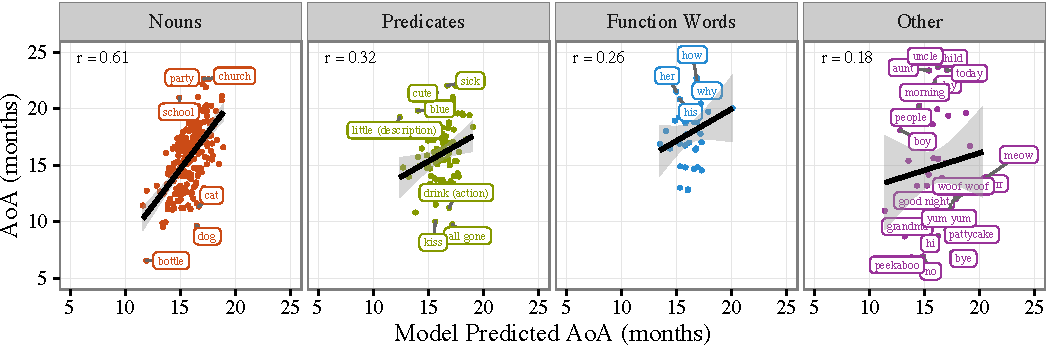
\includegraphics{figs/fit-1} 

}

\caption[English model fit]{English model fit.}\label{fig:fit}
\end{figure*}
\end{CodeChunk}

\section{Results}\label{results}

We fit a linear regression for each language's data, as well as a linear
mixed-effects model with language as a random effect for all the data
pooled. Figure \ref{fig:coefs} shows the magnitude of the coefficient
for each predictor in each language and cross-linguistically. We find
that frequency, concreteness, and babiness are relatively stronger
predictors of age of acquisition, across languages

\begin{CodeChunk}
\begin{figure*}[tb]

{\centering 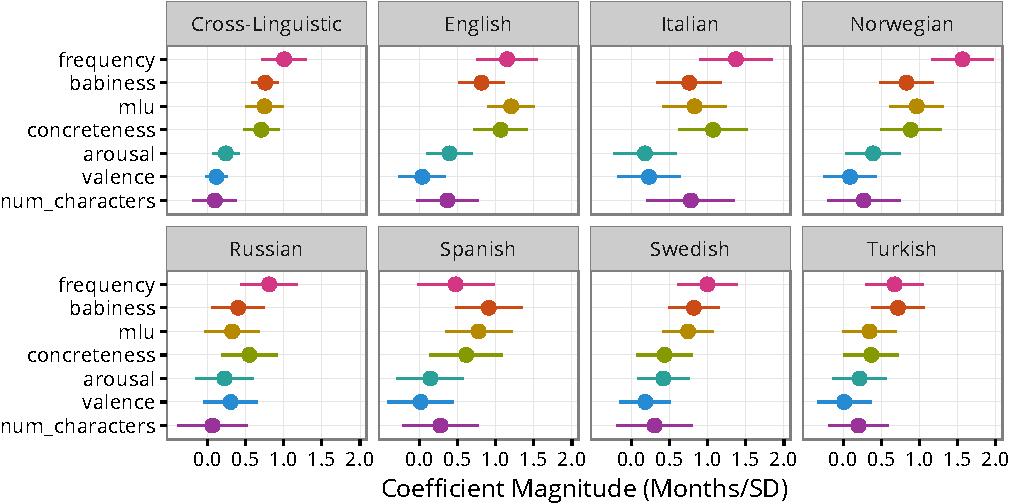
\includegraphics{figs/coefs-1} 

}

\caption[Magnitudes of predictor coefficients]{Magnitudes of predictor coefficients.}\label{fig:coefs}
\end{figure*}
\end{CodeChunk}

To assess developmental trends, we compare predictor values in two
groups of words to determine which features best distinguish words with
age of acquisition estimates earlier and later than 14 months. Within
English and across all languages, early learned words are distinguished
from later learned words on all of our measured factors (i.e.~they are
shorter, more concrete, etc). However, the magnitude of this difference
is especially large for frequency and babiness (Figure 2).

\section{Discussion}\label{discussion}

Overall, we find that while frequency is predictive of age of
acquisition across languages, conceptual factors are at least as
important, especially for the earliest learned words. Our results imply
that distributional theories of word learning should be constrained by
such conceptual factors, which are likely to apply across languages.

\section{Conclusion}\label{conclusion}

\section{Acknowledgements}\label{acknowledgements}

Thanks to the MacArthur-Bates CDI Advisory Board.

\section{References}\label{references}

\setlength{\parindent}{-0.1in} \setlength{\leftskip}{0.125in} \noindent

Bloom, P. (2002). \emph{How children learn the meanings of words}. MIT
press.

Brysbaert, M., Warriner, A. B., \& Kuperman, V. (2014). Concreteness
ratings for 40 thousand generally known english word lemmas.
\emph{Behavior Research Methods}, \emph{46}(3), 904--911.

Fenson, L. (2007). \emph{MacArthur-bates communicative development
inventories: User's guide and technical manual}. Paul H. Brookes
Publishing Company.

Goodman, J. C., Dale, P. S., \& Li, P. (2008). Does frequency count?
Parental input and the acquisition of vocabulary. \emph{Journal of Child
Language}, \emph{35}(3), 515.

MacWhinney, B. (2000). \emph{The cHILDES project: The database} (Vol.
2). Psychology Press.

Perry, L. K., Perlman, M., \& Lupyan, G. (2015). Iconicity in english
and spanish and its relation to lexical category and age of acquisition.
\emph{PloS One}, \emph{10}(9), e0137147.

Warriner, A. B., Kuperman, V., \& Brysbaert, M. (2013). Norms of
valence, arousal, and dominance for 13,915 english lemmas.
\emph{Behavior Research Methods}, \emph{45}(4), 1191--1207.

\end{document}
